\section{Fitting Diffusion Barriers using Neural Network}
\label{Chap:Al/Vac:section:NN}

The computational engine that provided the energetics used to evaluate energy differences and activation barriers before and after vacancy jump in Al 7075 alloy was the implementation of \ac{DFT} together with climbing image \acf{NEB} in the \ac{VASP} software with VTST package from Henkelman's group \cite{henkelman2000climbing,henkelman2000improved}. All-electron \ac{PAW} potentials were employed for the elemental constituents with the \ac{GGA} of \ac{PBE} for the exchange-correlation energy functional, $\mu_{xc}$, and the interpolation formula of Vosko et al. \cite{vosko1980accurate}. Using plane-wave cutoff energy of at 450.0 eV, the total energy for all models of initial and final images was converged to $10^{−7}$ eV/cell. The reciprocal space of bulk supercells was sampled with (2x2x2) k-point grids. Each grid was generated using the Monkhorst-Pack scheme \cite{monkhorst1976special}. A (4x4x4) conventional supercell with a single vacancy embedded was used for these calculations. For activation barrier calculations, 5 images between relaxed initial and final images were used. A spring constant was set to 5 $\text{eV}/\angstrom^2$. The force convergence criteria for all models was set to be less than 0.05 $\text{eV}/\angstrom$. The force-based quick-min optimizer was used to make \ac{NEB} calculations stable for high local concentration cases. \cite{sheppard2008optimization}

To sample a larger potential energy landscape, our \ac{NN} model training set contains mainly two different parts: 1) (4x4x4) randomly generated solid-solution structures with different local concentrations around jump pairs. 2) (2x2x2) randomly generated ordered structures embedded in (4x4x4) pure Al. The first training set is good for simulating vacancy diffusion of very early stage, during which Al alloy is in solid-solution state. The second training set is designed to accurately describe the behavior of vacancy moving across/along the boundary between solid-solution Al and ordered phases, and moving inside the ordered phases.


\begingroup
\begin{figure}[!ht]
  \centering
  \subfigure[]{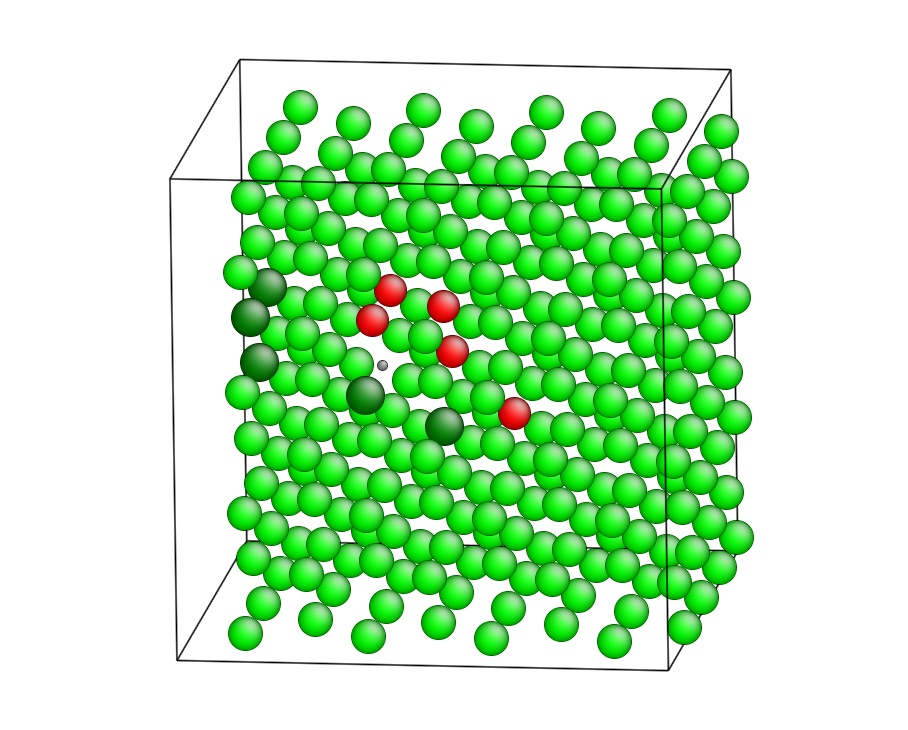
\includegraphics[width=0.49\linewidth]{Chap5/plots/ss_atomic.jpg}}
  \subfigure[]{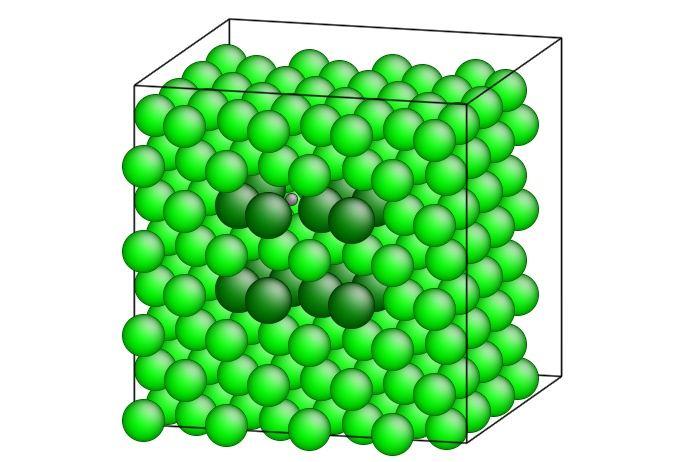
\includegraphics[width=0.49\linewidth]{Chap5/plots/ordered_atomic.jpg}}
\caption[Atomistic pictures of (4x4x4) supercells containing 256 atoms.]{Atomistic pictures of (4x4x4) supercells containing 256 atoms. (a) (b). color}
\label{Chap:Al/Vac:fig:atomic_illu}
\end{figure}
\endgroup






\newpage
\begingroup
\begin{figure}[!ht]
  \centering
  \subfigure{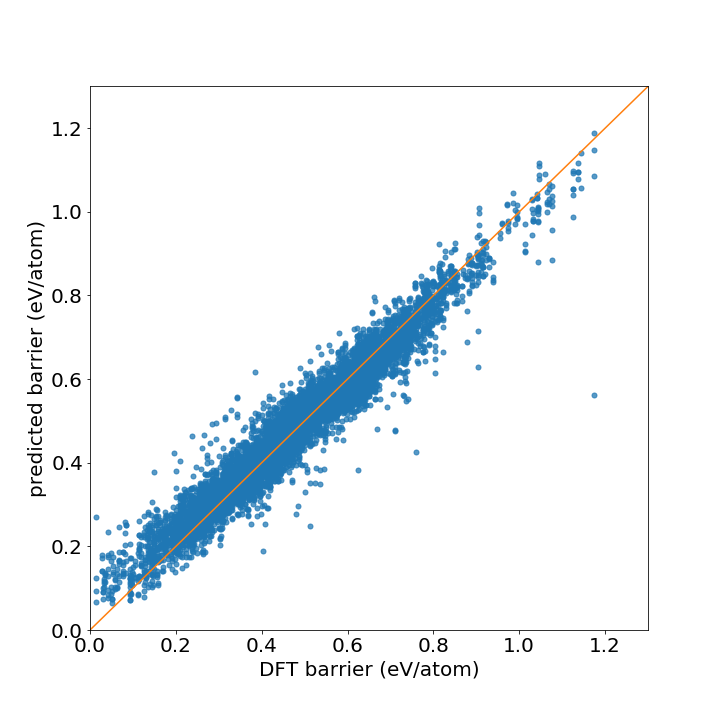
\includegraphics[width=0.49\linewidth]{Chap5/plots/total.png}}
  \subfigure{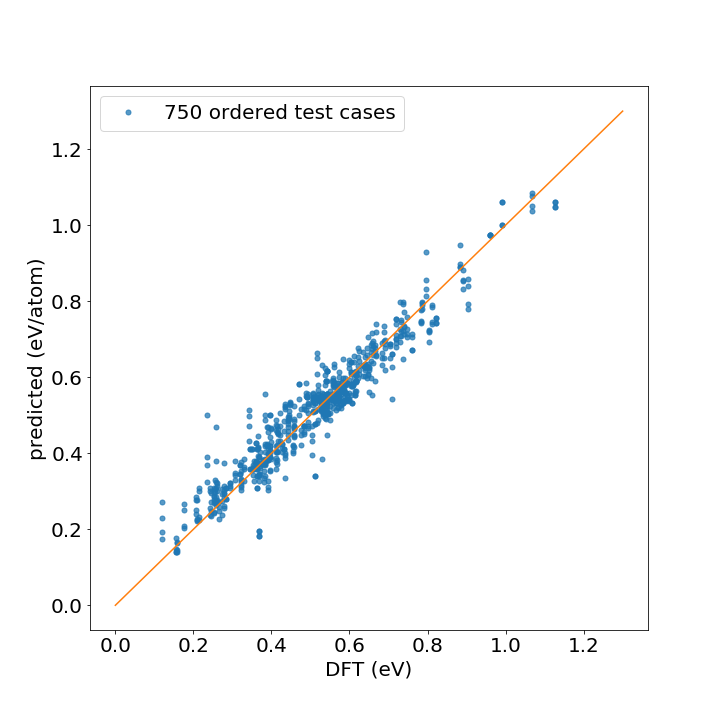
\includegraphics[width=0.49\linewidth]{Chap5/plots/fit_ordered.png}}
\caption[]{}
\label{Chap:Al/Vac:fig:fitting_all}
\end{figure}
\endgroup
